\documentclass{beamer}

\usetheme{Warsaw}
\usecolortheme{seahorse}
\setbeamertemplate{navigation symbols}{}
\setbeamertemplate{caption}{\raggedright\scriptsize\insertcaption\par}
\setbeamertemplate{headline}{%
\leavevmode%
    \begin{beamercolorbox}[wd=\paperwidth,ht=3ex,dp=1.9ex]{palette quaternary}%
    \insertsectionnavigationhorizontal{\paperwidth}{\hskip0pt plus1fill}{\hskip0pt plus1fill}
    \end{beamercolorbox}%
}
\setbeamercolor{background canvas}{bg=}
\setlength{\parskip}{\medskipamount} 

% \setbeamerfont{footnote}{size=\tiny}
\usepackage{beamerthemesplit}
\usepackage{lmodern}
\usepackage{bold-extra}
\usepackage{ragged2e}
\usepackage{pgf}
\usepackage{epsfig}
\usepackage{epstopdf}
\usepackage{graphicx}
\usepackage{slashbox}
\usepackage{amssymb}
\usepackage{xurl}
\usepackage{xcolor}
\usepackage{listings}
\usepackage{polski}
\usepackage[utf8]{inputenc}
\usepackage[absolute,overlay]{textpos}
\usepackage{graphicx}
\usepackage[style=numeric,backend=biber,sorting=none]{biblatex}
\usepackage[font=scriptsize,labelformat=empty,justification=centering]{caption}
\addbibresource{sdm2-1.bib}

\let\olditem=\item
\renewcommand{\item}{\olditem \justifying}

\apptocmd{\frame}{}{\justifying}{}

\newcommand{\C}{\emph{C}}
\newcommand{\CLogo}{\raisebox{-0.25\totalheight}{
\includegraphics[height=1.8\fontcharht\font`\B]{img/c-logo.png}}}
\newcommand{\Rust}{\emph{Rust}}
\newcommand{\RustLogo}{\raisebox{-0.25\totalheight}{
\includegraphics[height=1.8\fontcharht\font`\B]{img/rust-logo.png}}}
\newcommand{\Zig}{\emph{Zig}}
\newcommand{\ZigLogo}{\raisebox{-0.25\totalheight}{
\includegraphics[height=1.8\fontcharht\font`\B]{img/zig-logo.png}}}

\newcommand{\Modbus}{\emph{MODBUS\textsuperscript{\copyright}}}
\newcommand{\Lizard}{\lstinline{lizard}}

\newcommand{\IR}{\bbold R}
\def\Rset{\mathbb{R}}
\def\Zset{\mathbb{Z}}
\newcommand{\refbr}[1]{(\ref{#1})}
\newcommand{\beq}{\begin{equation}}
\newcommand{\eeq}{\end{equation}}
\newcommand{\und}[1]{\underline{#1}}
\newcommand\pro{\item[$+$]}
\newcommand\con{\item[$-$]}
\newcounter{saveenumi}
\newcommand{\seti}{\setcounter{saveenumi}{\value{enumi}}}
\newcommand{\conti}{\setcounter{enumi}{\value{saveenumi}}}
\lstset{
    numbers=left,
    breaklines=true,
    tabsize=2,
	numberstyle=\color{gray}\footnotesize,
    basicstyle=\small\ttfamily,
}
\newcommand{\ttbf}[1]{{\tt \textbf{#1}}}
% \AtBeginSection{
%   \begin{frame}
%   \vfill
%   \centering
%   \begin{beamercolorbox}[sep=8pt,center,shadow=true,rounded=true]{title}
%     \usebeamerfont{title}\insertsectionhead\par%
%   \end{beamercolorbox}
%   \vfill
%   \end{frame}
% }

\hypersetup{
   pdftitle={Analiza wybranych języków programowania na systemy wbudowane pod kątem wydajności i niezawodności},
   pdfauthor={Jakub Ostrzołek},
   pdfborder={0 0 0}
}

\title[Analiza języków dla systemów wbudowanych \insertframenumber/\inserttotalframenumber]{
	 Analiza wybranych języków programowania na systemy wbudowane pod
	 kątem wydajności i niezawodności
}
\author[Jakub Ostrzołek]{
 	\textbf{Jakub Ostrzołek} \\ \vspace{\smallskipamount}
	\scriptsize Kierunek: Informatyka, Inteligentne Systemy \\ \vspace{\bigskipamount}
  \footnotesize Promotor: dr inż. Patryk Chaber
}

\institute{
	Instytut Automatyki i Informatyki Stosowanej \\%
  Politechnika Warszawska
}

\begin{document}

\frame{\titlepage}

% \frame{\tableofcontents\frametitle{Plan prezentacji}}

\section{Motywacja}

\begin{frame}
	\frametitle{Motywacja}

	\begin{columns}
		\begin{column}{.60\textwidth}
			\justifying
			Język C wciąż zdecydowanie dominuje w zastosowaniach
			systemów wbudowanych.

			\begin{itemize}
				\item Z czego wynika ta sytuacja?
				\item Z jakimi zaletami i problemami wiąże się zastosowanie
				      nowoczesnych języków?
				\item Niewiele badań na ten temat.
			\end{itemize}

		\end{column}
		\begin{column}{.40\textwidth}
			\begin{figure}
				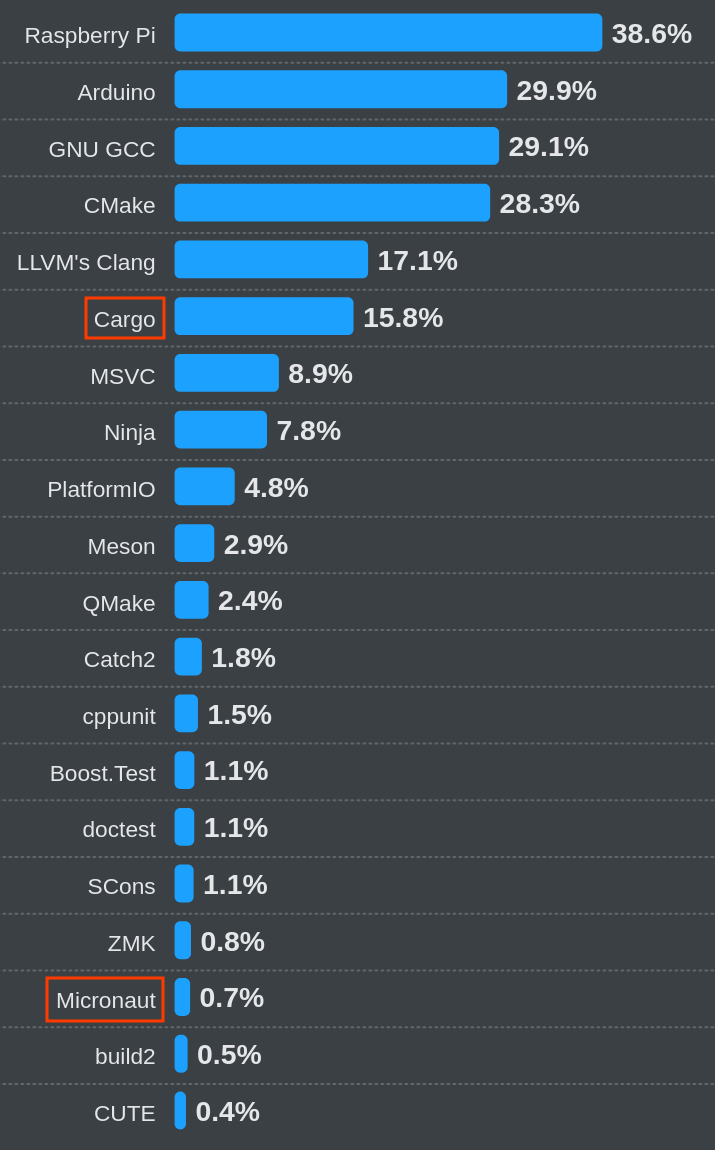
\includegraphics[height=0.7\textheight]{img/so-survey.png}
				\centering
				\caption{\citetitle{so-survey} \cite{so-survey}}
			\end{figure}
		\end{column}
	\end{columns}
\end{frame}

\section{Cele pracy}

\begin{frame}
	\frametitle{Cele pracy}
	Porównanie ilościowe i jakościowe języków w praktycznych
	zastosowaniach dla systemów wbudowanych pod kątem:

	\begin{itemize}
		\item wydajności (np. czas wykonania, zajętość pamięci),
		\item bezpieczeństwa (np. zabezpieczenia kompilatora, narzędzia do
		      statycznej analizy),
		\item udogodnień programisty (np. dostępność bibliotek, łatwość
		      użytkowania systemu budowania).
	\end{itemize}

	Wybrane języki do analizy: \C{} (\CLogo{}), \Rust{} (\RustLogo{}), \Zig{} (\ZigLogo{}).
\end{frame}

\section{Zakres pracy i osiągnięcia}

\begin{frame}
	\frametitle{Zakres pracy i osiągnięcia}
	\begin{enumerate}
		\item {\color{gray} Opracowanie metod i metryk porównania języków, w tym:
		      \label{item:methods}}
		      \begin{itemize}
			      \color{gray}
			      \item rozszerzenie narzędzia \Lizard{} o wsparcie dla
			            języka \Zig{}.
		      \end{itemize}
		\item Implementacja zbioru przykładowych układów elektronicznych oraz
		      programów w każdym z rozważanych języków:
		      \begin{enumerate}[A]
			      \item {\color{gray} kontrola diody LED \; \CLogo{}\checkmark{}
			            \RustLogo{}\checkmark{} \ZigLogo{}\checkmark{},}
			      \item {\color{gray} kontrola silnika za pomocą potencjometru \;
			            \CLogo{}\checkmark{} \RustLogo{}\checkmark{}
			            \ZigLogo{}\checkmark{},}
			      \item {\color{gray} regulacja PID obrotów silnika z komunikacją
			            protokołem \linebreak \Modbus{} \; \CLogo{}\checkmark{}
			            \RustLogo{}\checkmark,} \label{item:controller-start}
			      \item regulacja DMC obrotów silnika z komunikacją
			            protokołem \linebreak \Modbus{}. \label{item:controller-end}
		      \end{enumerate}
		      Realizacja w wersji z {\color{gray} systemem operacyjnym} oraz bez.
		\item {\color{gray} Implementacja panelu sterowania regulatorem z zadań
		      \ref{item:controller-start}-\ref{item:controller-end}.}
		\item Zastosowanie metod z pkt. \ref{item:methods} do każdego z
		      programów.
		\item Zestawienie wyników porównania (w postaci tabel, wykresów).
	\end{enumerate}
\end{frame}

% \section{Osiągnięcia}
%
% \begin{frame}
% 	\frametitle{Osiągnięcia}
% 	\begin{enumerate}
% 		\item Opracowanie miar ilościowych do porównywania języków, w tym:
% 		      \begin{itemize}
% 			      \item rozszerzenie biblioteki \Lizard{} o wsparcie dla
% 			            języka \Zig{}.
% 		      \end{itemize}
% 		\item Implementacja programów przykładowych (w wersji z systemem
% 		      operacyjnym):
% 		      \begin{enumerate}[A]
% 			      \item kontrola diody LED (\CLogo{}, \RustLogo{}, \ZigLogo{}),
% 			      \item kontrola silnika za pomocą potencjometru
% 			            (\CLogo{}, \RustLogo{}, \ZigLogo{}),
% 			      \item regulacja PID obrotów silnika z komunikacją
% 			            protokołem \linebreak \Modbus{} (\RustLogo{}).
% 			            \label{item:controller}
% 		      \end{enumerate}
% 		\item Realizacja układów do wykonania powyższych zadań.
% 		\item Implementacja panelu sterowania regulatorem z zadania \ref{item:controller}.
% 	\end{enumerate}
% \end{frame}

\section{Plan przyszłych prac}

\begin{frame}
	\frametitle{Plan przyszłych prac}

	\begin{enumerate}
		\item Implementacja programów przykładowych (w wersji z
		      systemem operacyjnym): \label{item:tasks-no-os}
		      \begin{enumerate}[A]
			      \setcounter{enumii}{2}
			      \item \textbf{marzec:} regulacja PID obrotów silnika z komunikacją
			            protokołem \Modbus{} \; \ZigLogo{},
			      \item \textbf{marzec:} regulacja DMC obrotów silnika z
			            komunikacją protokołem \Modbus{} \; \CLogo{}\, \RustLogo{}\,
			            \ZigLogo{}.
		      \end{enumerate}
		      % \item {\color{gray} Opracowanie miar ilościowych do porównywania języków.}
		      % \item Implementacja programów przykładowych (w wersji z systemem
		      %       operacyjnym):
		      %       \begin{enumerate}[A]
		      % 	      \item {\color{gray}kontrolowanie diody LED [\C{}, \Rust{},
		      % 			            \Zig{}],}
		      % 	      \item {\color{gray}kontrolowanie obrotów silnika za pomocą
		      % 	            potencjometru [\C{}, \Rust{}, \Zig{}],}
		      % 	      \item \textbf{Marzec:} {\color{gray}regulacja PID obrotów
		      % 		            silnika z komunikacją protokołem \Modbus{}} [\C{},
		      % 		            {\color{gray}\Rust{}}, \Zig{}],
		      % 	      \item \textbf{Marzec:} regulacja DMC obrotów silnika z
		      % 	            komunikacją protokołem \Modbus{} [\C{}, \Rust{}, \Zig{}],
		      %       \end{enumerate}
		      % \item {\color{gray}Realizacja układów do wykonania powyższych
		      %       zadań.}
		      % \item {\color{gray}Implementacja panelu sterowania regulatorem z zadań
		      %       C-D.}
		\item \textbf{kwiecień:} Implementacja programów z pkt.
		      \ref{item:tasks-no-os} w wersji bez systemu operacyjnego.
		\item \textbf{kwiecień:} Pomiary metryk i analiza wyników.
		\item \textbf{maj-czerwiec:} Sporządzenie dokumentu pracy
		      magisterskiej.
	\end{enumerate}
\end{frame}

\begin{frame}[allowframebreaks,noframenumbering]
	\frametitle{Bibliografia}
	\nocite{*} % Print all entries
	\printbibliography[heading=none]
\end{frame}

% \begin{frame}
% 	\frametitle{Halma}
% 	\begin{columns}
% 		\begin{column}{.48\textwidth}
% 			\begin{itemize}
% 				\item Cel -- ustawić wszystkie piony na polu startowym przeciwnika
% 				\item Poruszanie o 1 pole
% 				\item Przeskakiwanie przez 1 piona (dozwolone łączenie wiele na raz)
% 			\end{itemize}
% 		\end{column}%
% 		\hfill
% 		\begin{column}{.60\textwidth}
% 			\begin{figure}
% 				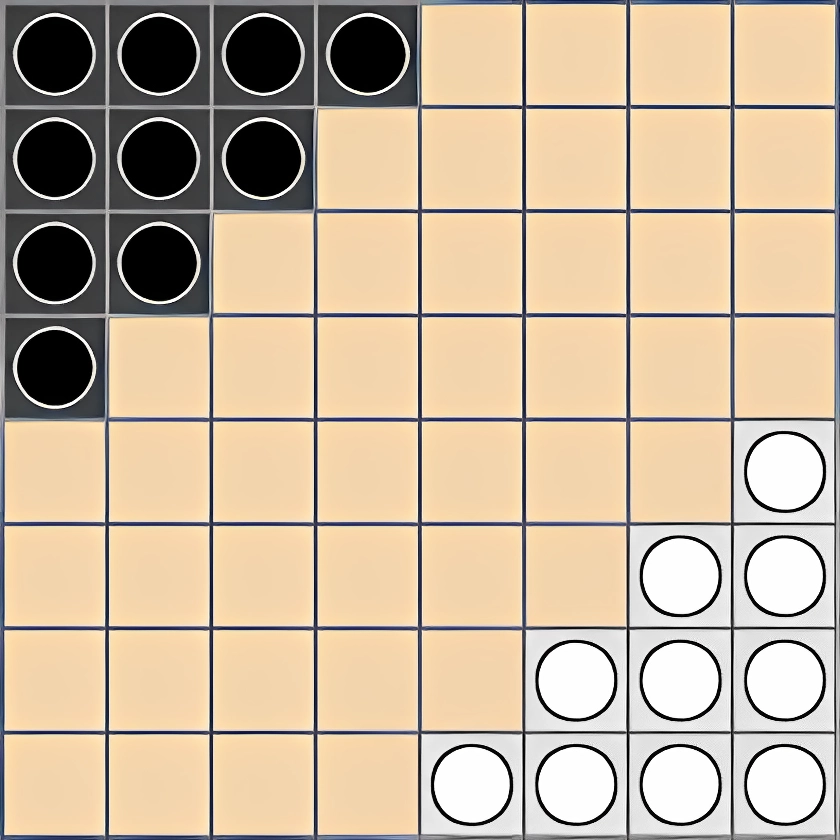
\includegraphics[height=4.5cm]{img/halma.png}
% 				\centering
% 				\caption{\url{https://brainking.com/en/GameRules?tp=33}}
% 			\end{figure}
% 		\end{column}
% 	\end{columns}
% \end{frame}

% \begin{frame}
% 	\frametitle{Dōbutsu shōgi}
% 	\begin{columns}
% 		\begin{column}{.48\textwidth}
% 			\begin{itemize}
% 				\item Cel -- zbić lwa przeciwnika lub przejść lwem na stronę przeciwnika
% 				\item Poruszanie zgodnie z oznaczeniami na figurach
% 				\item Promocja kurczaka do kury
% 				\item Możliwość stawiania zbitych figur przeciwnika jako swoich
% 			\end{itemize}
% 		\end{column}%
% 		\hfill
% 		\begin{column}{.60\textwidth}
% 			\begin{figure}
% 				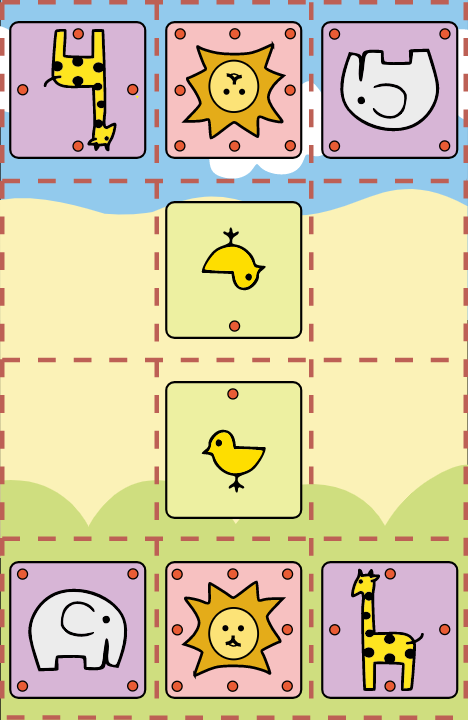
\includegraphics[height=4.5cm]{img/dobutsu-shogi.png}
% 				\centering
% 				\caption{\url{https://www.pychess.org/variants/dobutsu}}
% 			\end{figure}
% 		\end{column}
% 	\end{columns}
% \end{frame}

% \begin{frame}
% 	\frametitle{Silnik gry}
% 	\begin{columns}
% 		\begin{column}{.50\textwidth}
% 			Silnik gry -- automat
% 			\begin{itemize}
% 				\item odseparowany od modułu dekodującego zasady
% 				\item inicjalizowany stanem początkowym pochodzącym z modułu dekodującego zasady
% 				\item dla każdego stanu generuje możliwe przejścia
% 				\item dobrze przetestowany
% 			\end{itemize}
% 		\end{column}%
% 		\hfill
% 		\begin{column}{.50\textwidth}
% 			\begin{figure}
% 				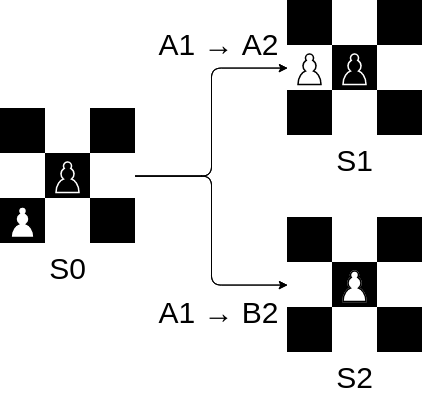
\includegraphics[width=4.5cm]{img/stany.png}
% 				\centering
% 			\end{figure}
% 		\end{column}
% 	\end{columns}
% \end{frame}

% \begin{frame}
% 	\frametitle{Interfejs użytkownika}
% 	\begin{itemize}
% 		\item Tematycznie najmniej istotna część projektu
% 		\item Wersja minimalna
% 		      \begin{itemize}
% 			      \item interfejs terminalowy
% 			      \item rozgrywka na jednym urządzeniu
% 		      \end{itemize}
% 		\item Wersja docelowa
% 		      \begin{itemize}
% 			      \item interfejs w przeglądarce internetowej
% 			      \item komunikacja z serwerem, na którym działa silnik gry (po protokole HTTP/WS)
% 			      \item rozgrywka poprzez 2 urządzenia
% 		      \end{itemize}
% 	\end{itemize}
% \end{frame}


% \begin{frame}[fragile]
% 	\frametitle{BGD -- BoardGameDescription\addtocounter{footnote}{-1}\footnotemark}
% 	\stepcounter{footnote}
% 	\begin{columns}
% 		\begin{column}{.5\textwidth}
% 			\begin{itemize}
% 				\item Cel: możliwość opisu jak największej liczby gier
% 				\item Opis gry za pomocą abstrakcyjnych elementów składowych (np. obiekt, lokacja, widoczność)
% 				\item Mało zwięzły (Chińczyk: 400 linii, Manilla: 1100 linii)
% 				\item Brak pętli, list, itp.
% 			\end{itemize}
% 		\end{column}%
% 		\hfill
% 		\begin{column}{.5\textwidth}
% 			\begin{lstlisting}
% Locations {
%  Loc1 {Startspace=true;}
%  Loc2 ...  }
% LocationConnections {
%  Directed {Loc1 Loc2} }
% Objects {
%  Pawn {...}
%  Dice {...} }
% Rounds {
%  Main() {...}
%  ... }
% Actions {
%  StartPawn(Location l) {...}
%  ... }
% 			\end{lstlisting}
% 		\end{column}
% 	\end{columns}
% 	\footcitetext{BGD}
% \end{frame}

% \begin{frame}
% 	\frametitle{RAS -- Rule Automation System\cite{RAS}}
% 	\begin{itemize}
% 		\item Język opisu gier karcianych
% 		\item Główny cel: używanie przez ludzi niezaznajomionych z programowaniem
% 		\item Ograniczony tylko do gier karcianych
% 		\item Brak udogodnień znanych z języków programowania (np. pętle, listy)
% 	\end{itemize}
% \end{frame}

% \begin{frame}
% 	\frametitle{Metagame\cite{metagame}}
% 	\begin{itemize}
% 		\item Język opisu gier opartych o szachownicę
% 		\item Główny cel: dokładny opis gier na potrzeby zadań SI
% 		\item Bardzo rozbudowany, wiele elementów składowych języka
% 		\item Skomplikowany w pisaniu i rozumieniu
% 	\end{itemize}
% \end{frame}

% \begin{frame}[fragile]
% 	\frametitle{GDL -- Game Description Language\addtocounter{footnote}{-1}\footnotemark}
% 	\stepcounter{footnote}
% 	\begin{columns}
% 		\begin{column}{.50\textwidth}
% 			\begin{itemize}
% 				\item Cel: opis gier do zadań SI
% 				\item Predykaty głównym budulcem zasad %(podobny do Prologa)
% 				\item Bardzo elastyczny, przy tym mało skomplikowany
% 				\item Brak konceptów z gier planszowych (plansza, gracz, itp.)
% 				\item Brak operacji arytmetycznych
% 			\end{itemize}
% 		\end{column}%
% 		\hfill
% 		\begin{column}{.50\textwidth}
% 			\begin{lstlisting}
% (role xplayer)
% (role oplayer)
% (<=(legal ?player (mark ?m ?n))
%  (true (cell ?m ?n blank))
%  (true (control ?player)))
% (<=(next (cell ?m ?n x))
%  (does xplayer (mark ?m ?n)))
% (<= terminal (line x))
% (<= (goal xplayer 100)
%  (line x))
% 			\end{lstlisting}
% 		\end{column}
% 	\end{columns}
% 	\footcitetext{GDL}
% \end{frame}

% \begin{frame}
% 	\frametitle{Podsumowanie istniejących rozwiązań}
% 	\begin{itemize}
% 		\item Istnieją rozwiązania spełniające cele mojego projektu
% 		\item Skupiają się na wykorzystaniu w zadaniach SI
% 		\item Mało przyjazne dla użytkownika definiującego zasady
% 		\item Wymagają doświadczonego programisty do opisu zasad
% 	\end{itemize}
% \end{frame}

% \begin{frame}
% 	\frametitle{Schemat systemu}
% 	\begin{figure}
% 		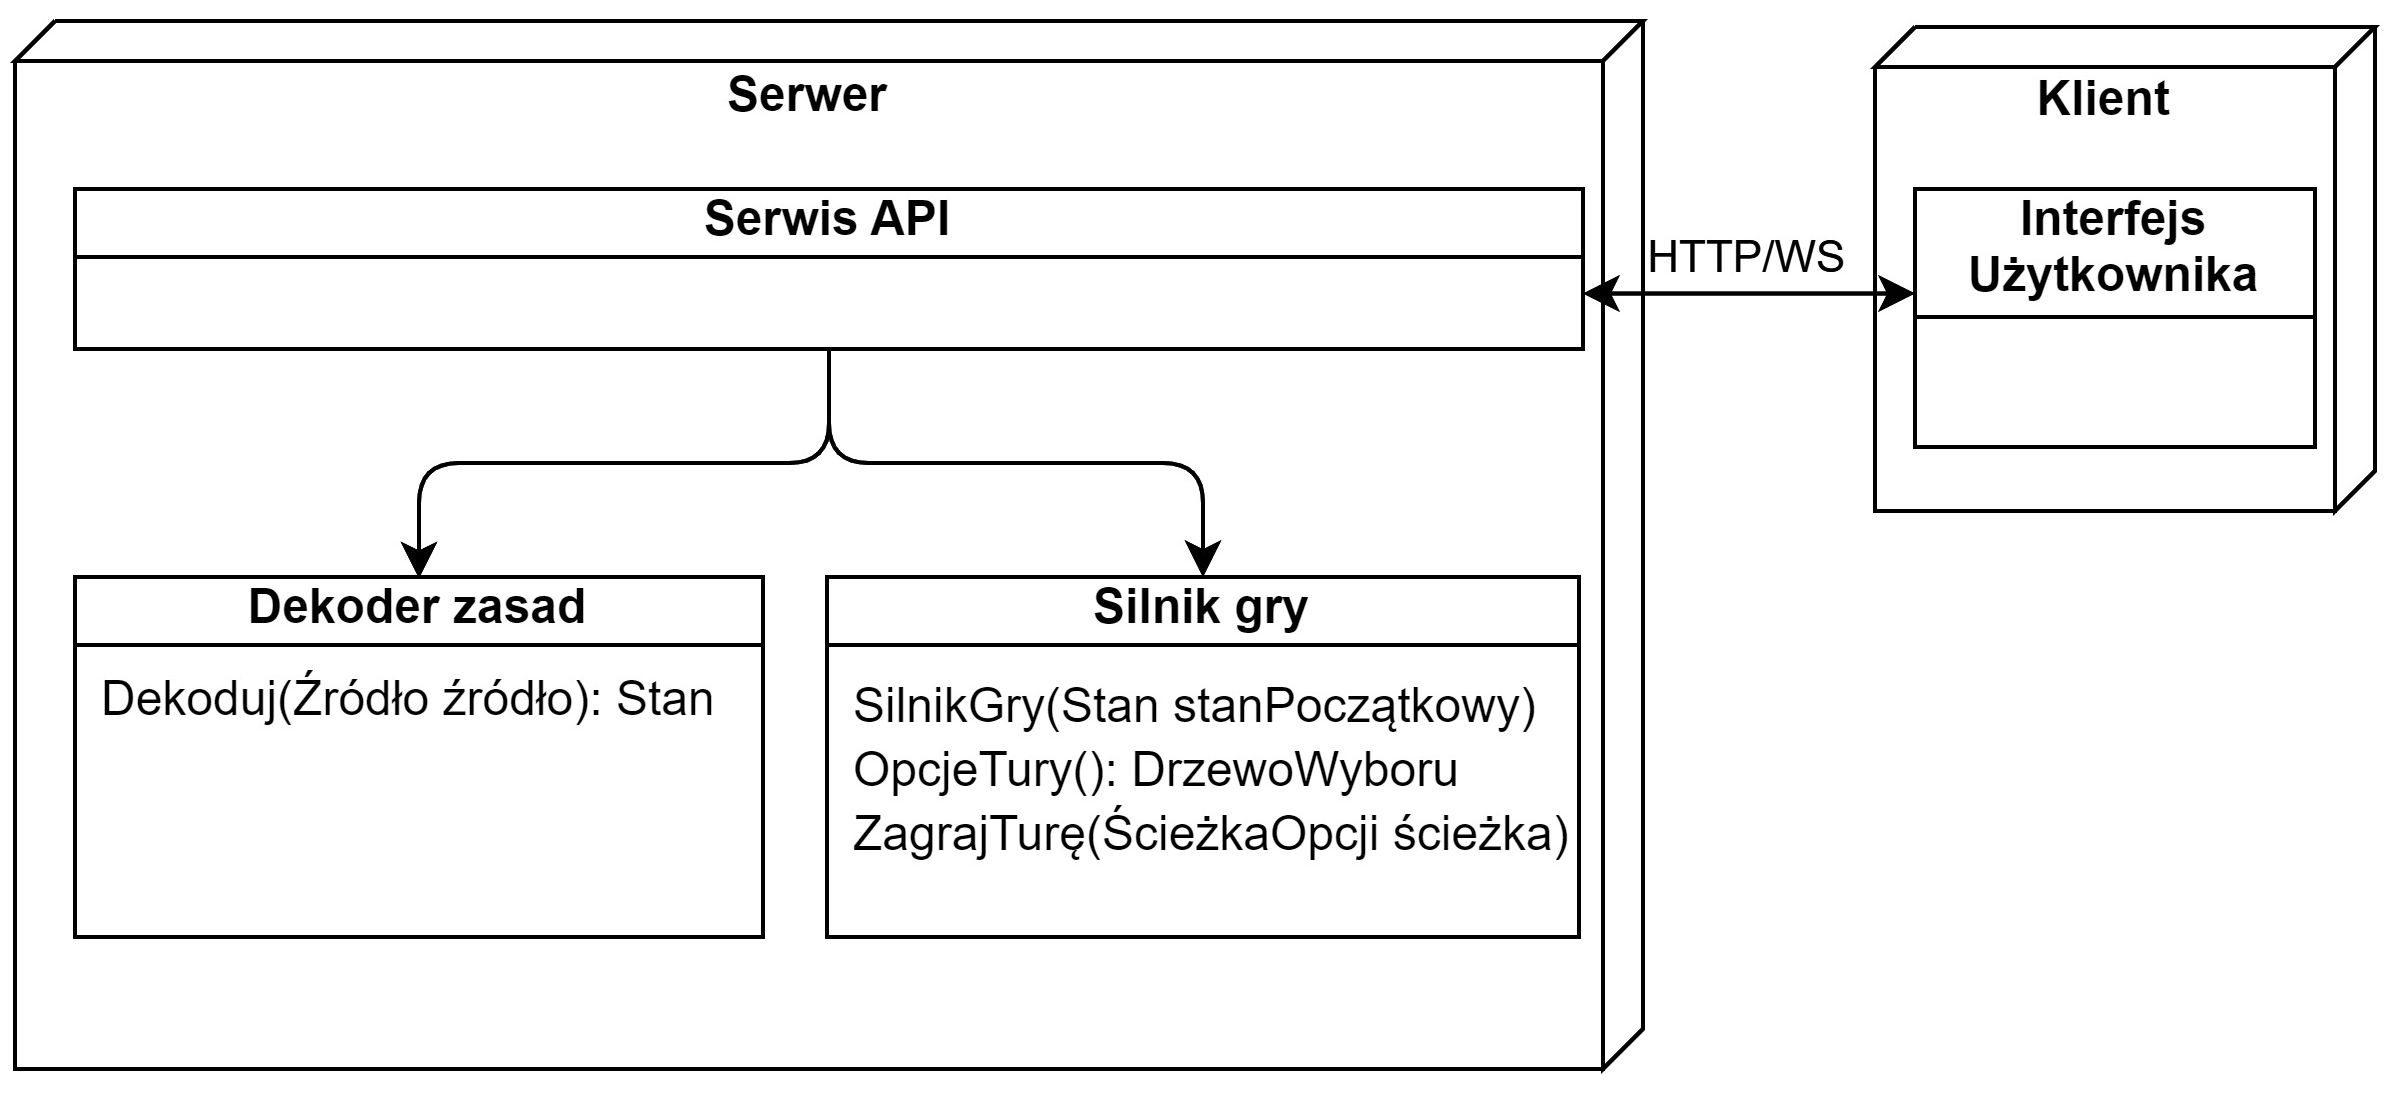
\includegraphics[height=5cm]{img/mess-system-diagram.jpg}
% 		\centering
% 	\end{figure}
% \end{frame}
%
% \begin{frame}
% 	\frametitle{Język -- elementy}
% 	\begin{itemize}
% 		\item rozmiar planszy: \ttbf{(int, int)}
% 		\item ustawienie początkowe: \ttbf{Mapa<Pozycja, Figura>}
% 		\item przebieg tury
% 		      \begin{itemize}
% 			      \item funkcja wyboru: \ttbf{() $\Rightarrow$ DrzewoWyboru}
% 			      \item akcja: \ttbf{(ŚcieżkaOpcji) $\Rightarrow$ void}
% 		      \end{itemize}
% 		\item definicja typów figur
% 		      \begin{itemize}
% 			      \item generatory ruchu: \ttbf{(Pozycja) $\Rightarrow$ []Pozycja}
% 			      \item funkcje wyboru: \ttbf{(Pozycja) $\Rightarrow$ DrzewoWyboru}
% 			      \item akcje: \ttbf{(Pozycja, ŚcieżkaOpcji) $\Rightarrow$ void}
% 		      \end{itemize}
% 		\item walidatory stanu gry po ruchu: \ttbf{(Ruch) $\Rightarrow$ bool}
% 		\item funkcja końca gry: \ttbf{() $\Rightarrow$ (bool, Gracz)}
% 		\item bieżący stan gry dostępny z każdej funkcji (tylko do odczytu)
% 		\item kilka funkcji wbudowanych modyfikujących stan gry (np. \ttbf{capture}, \ttbf{move})
% 	\end{itemize}
% \end{frame}
%
% \begin{frame}
% 	\frametitle{Interakcja z użytkownikiem -- drzewo wyboru}
% 	\begin{figure}
% 		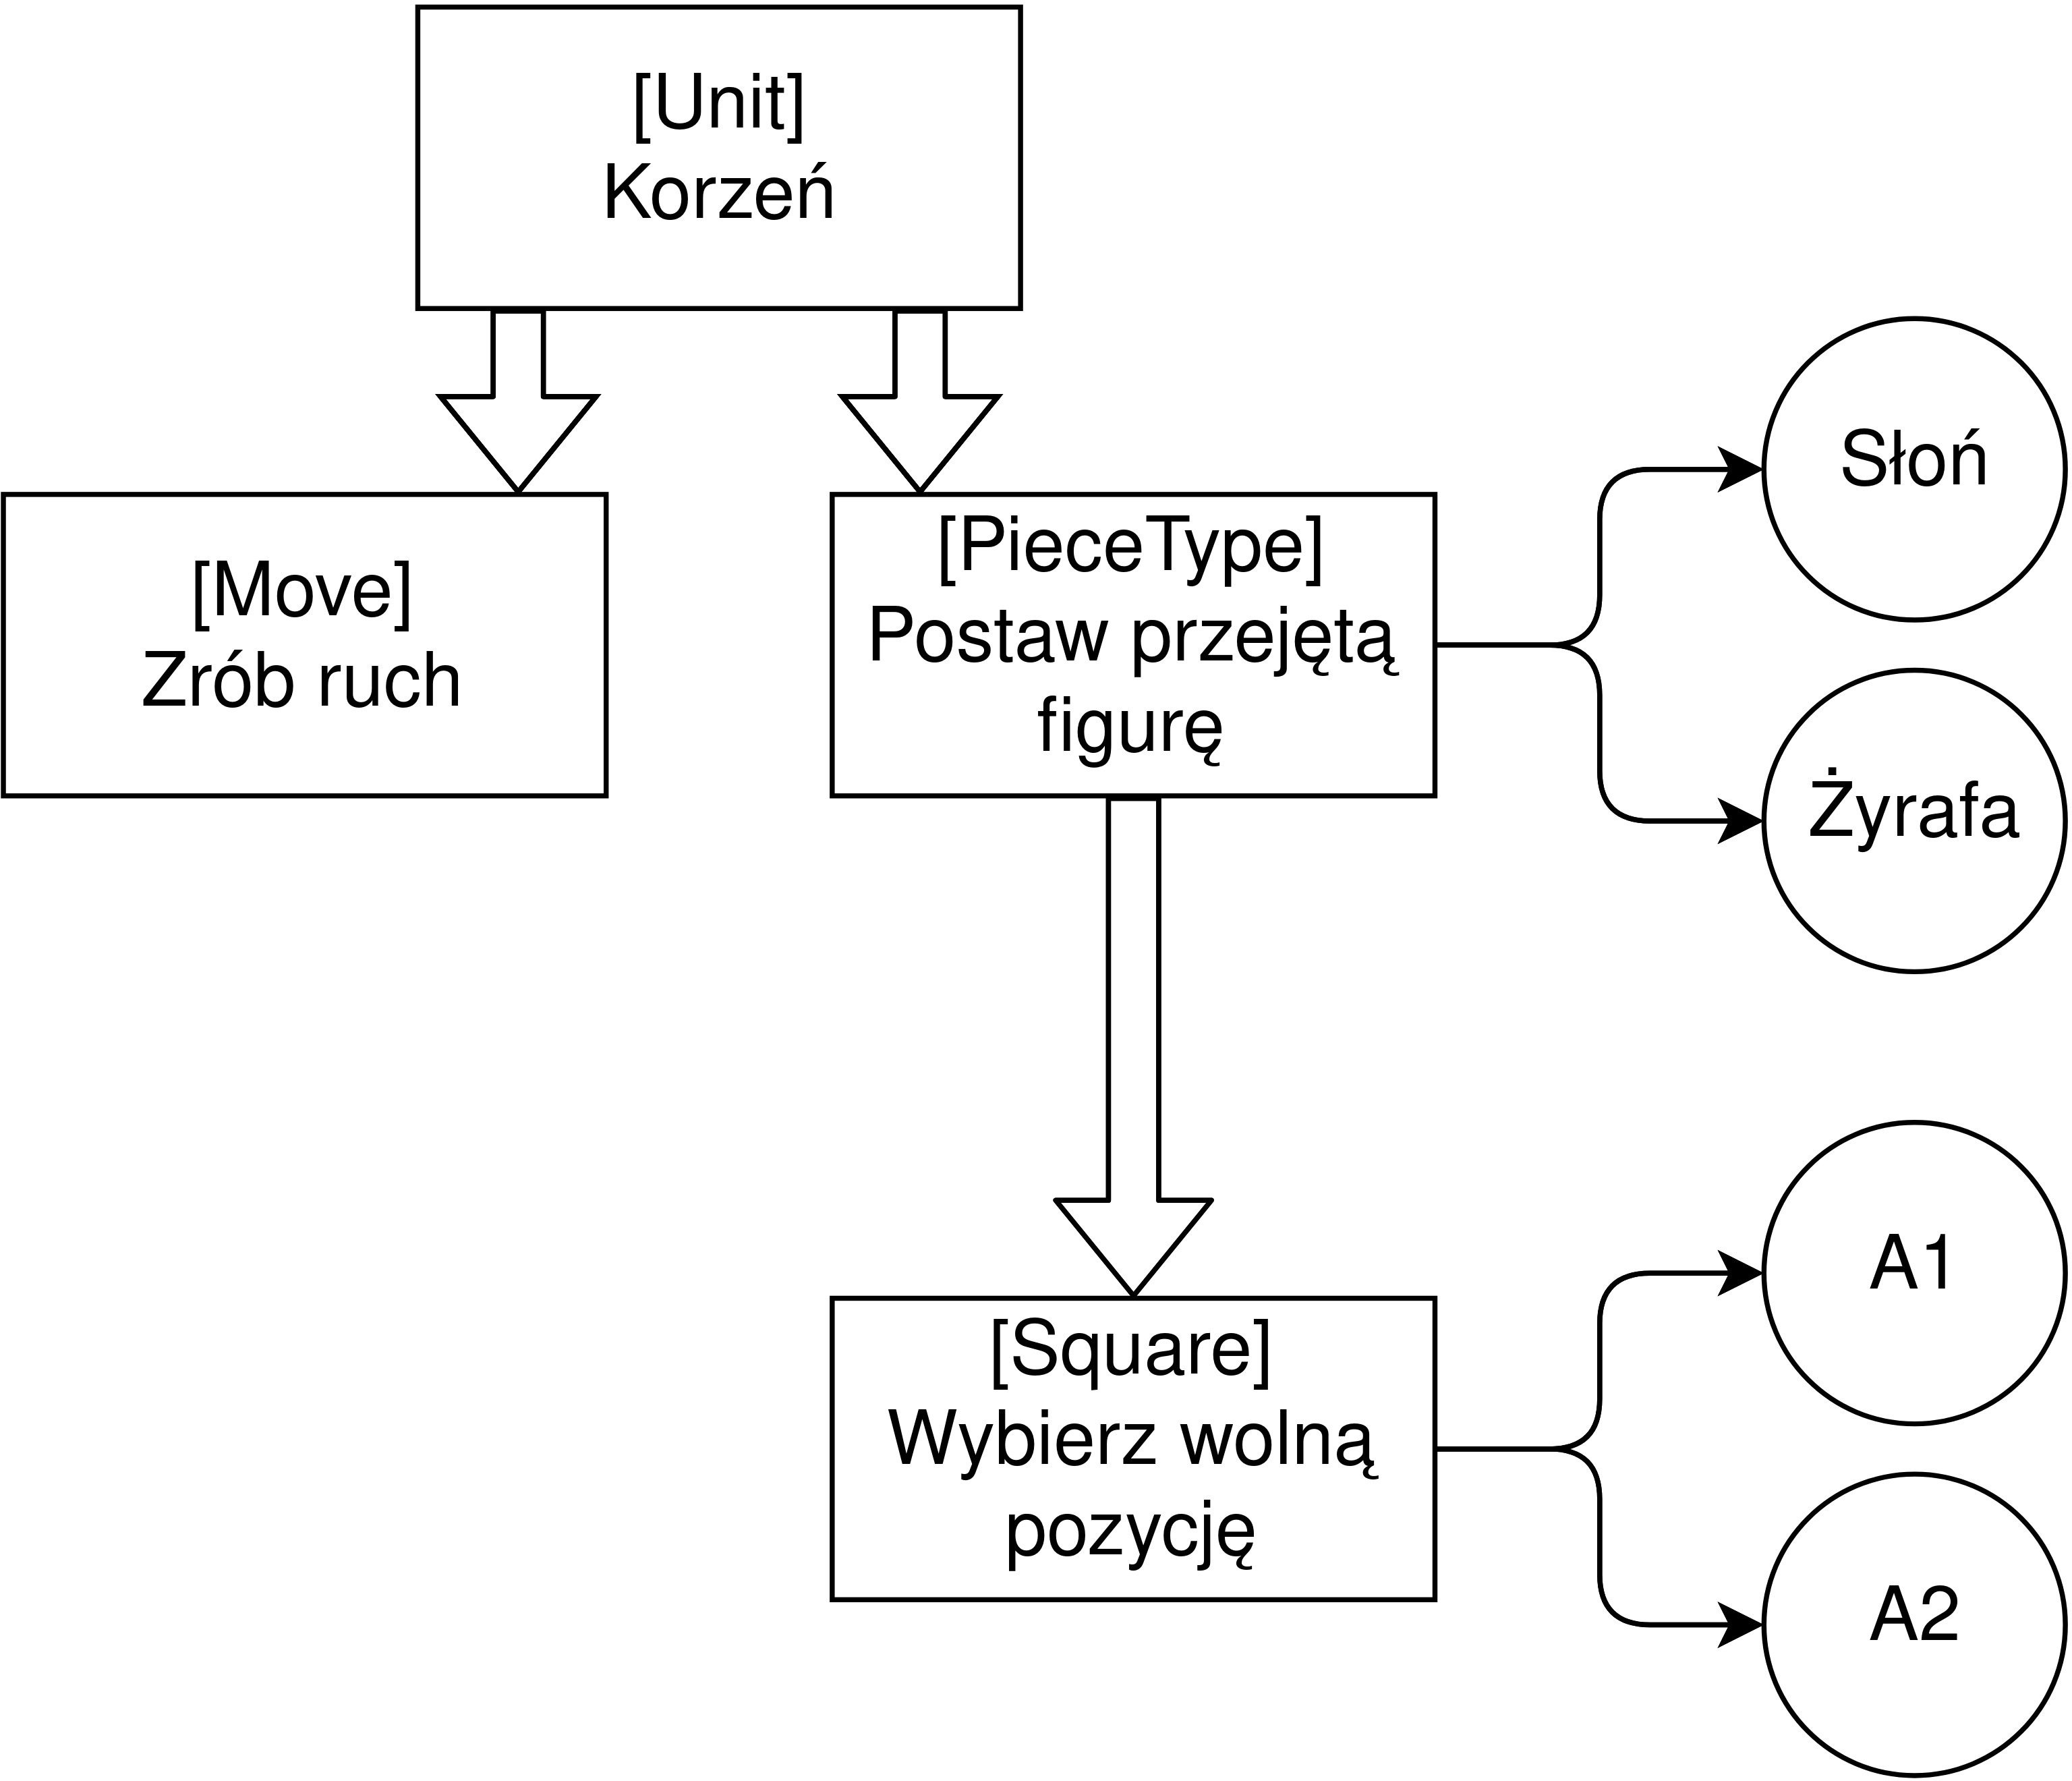
\includegraphics[height=7cm]{img/mess-choice-diagram.jpg}
% 		\centering
% 	\end{figure}
% \end{frame}
%
% \begin{frame}[noframenumbering]
% 	\frametitle{Interakcja z użytkownikiem -- drzewo opcji}
% 	\begin{figure}
% 		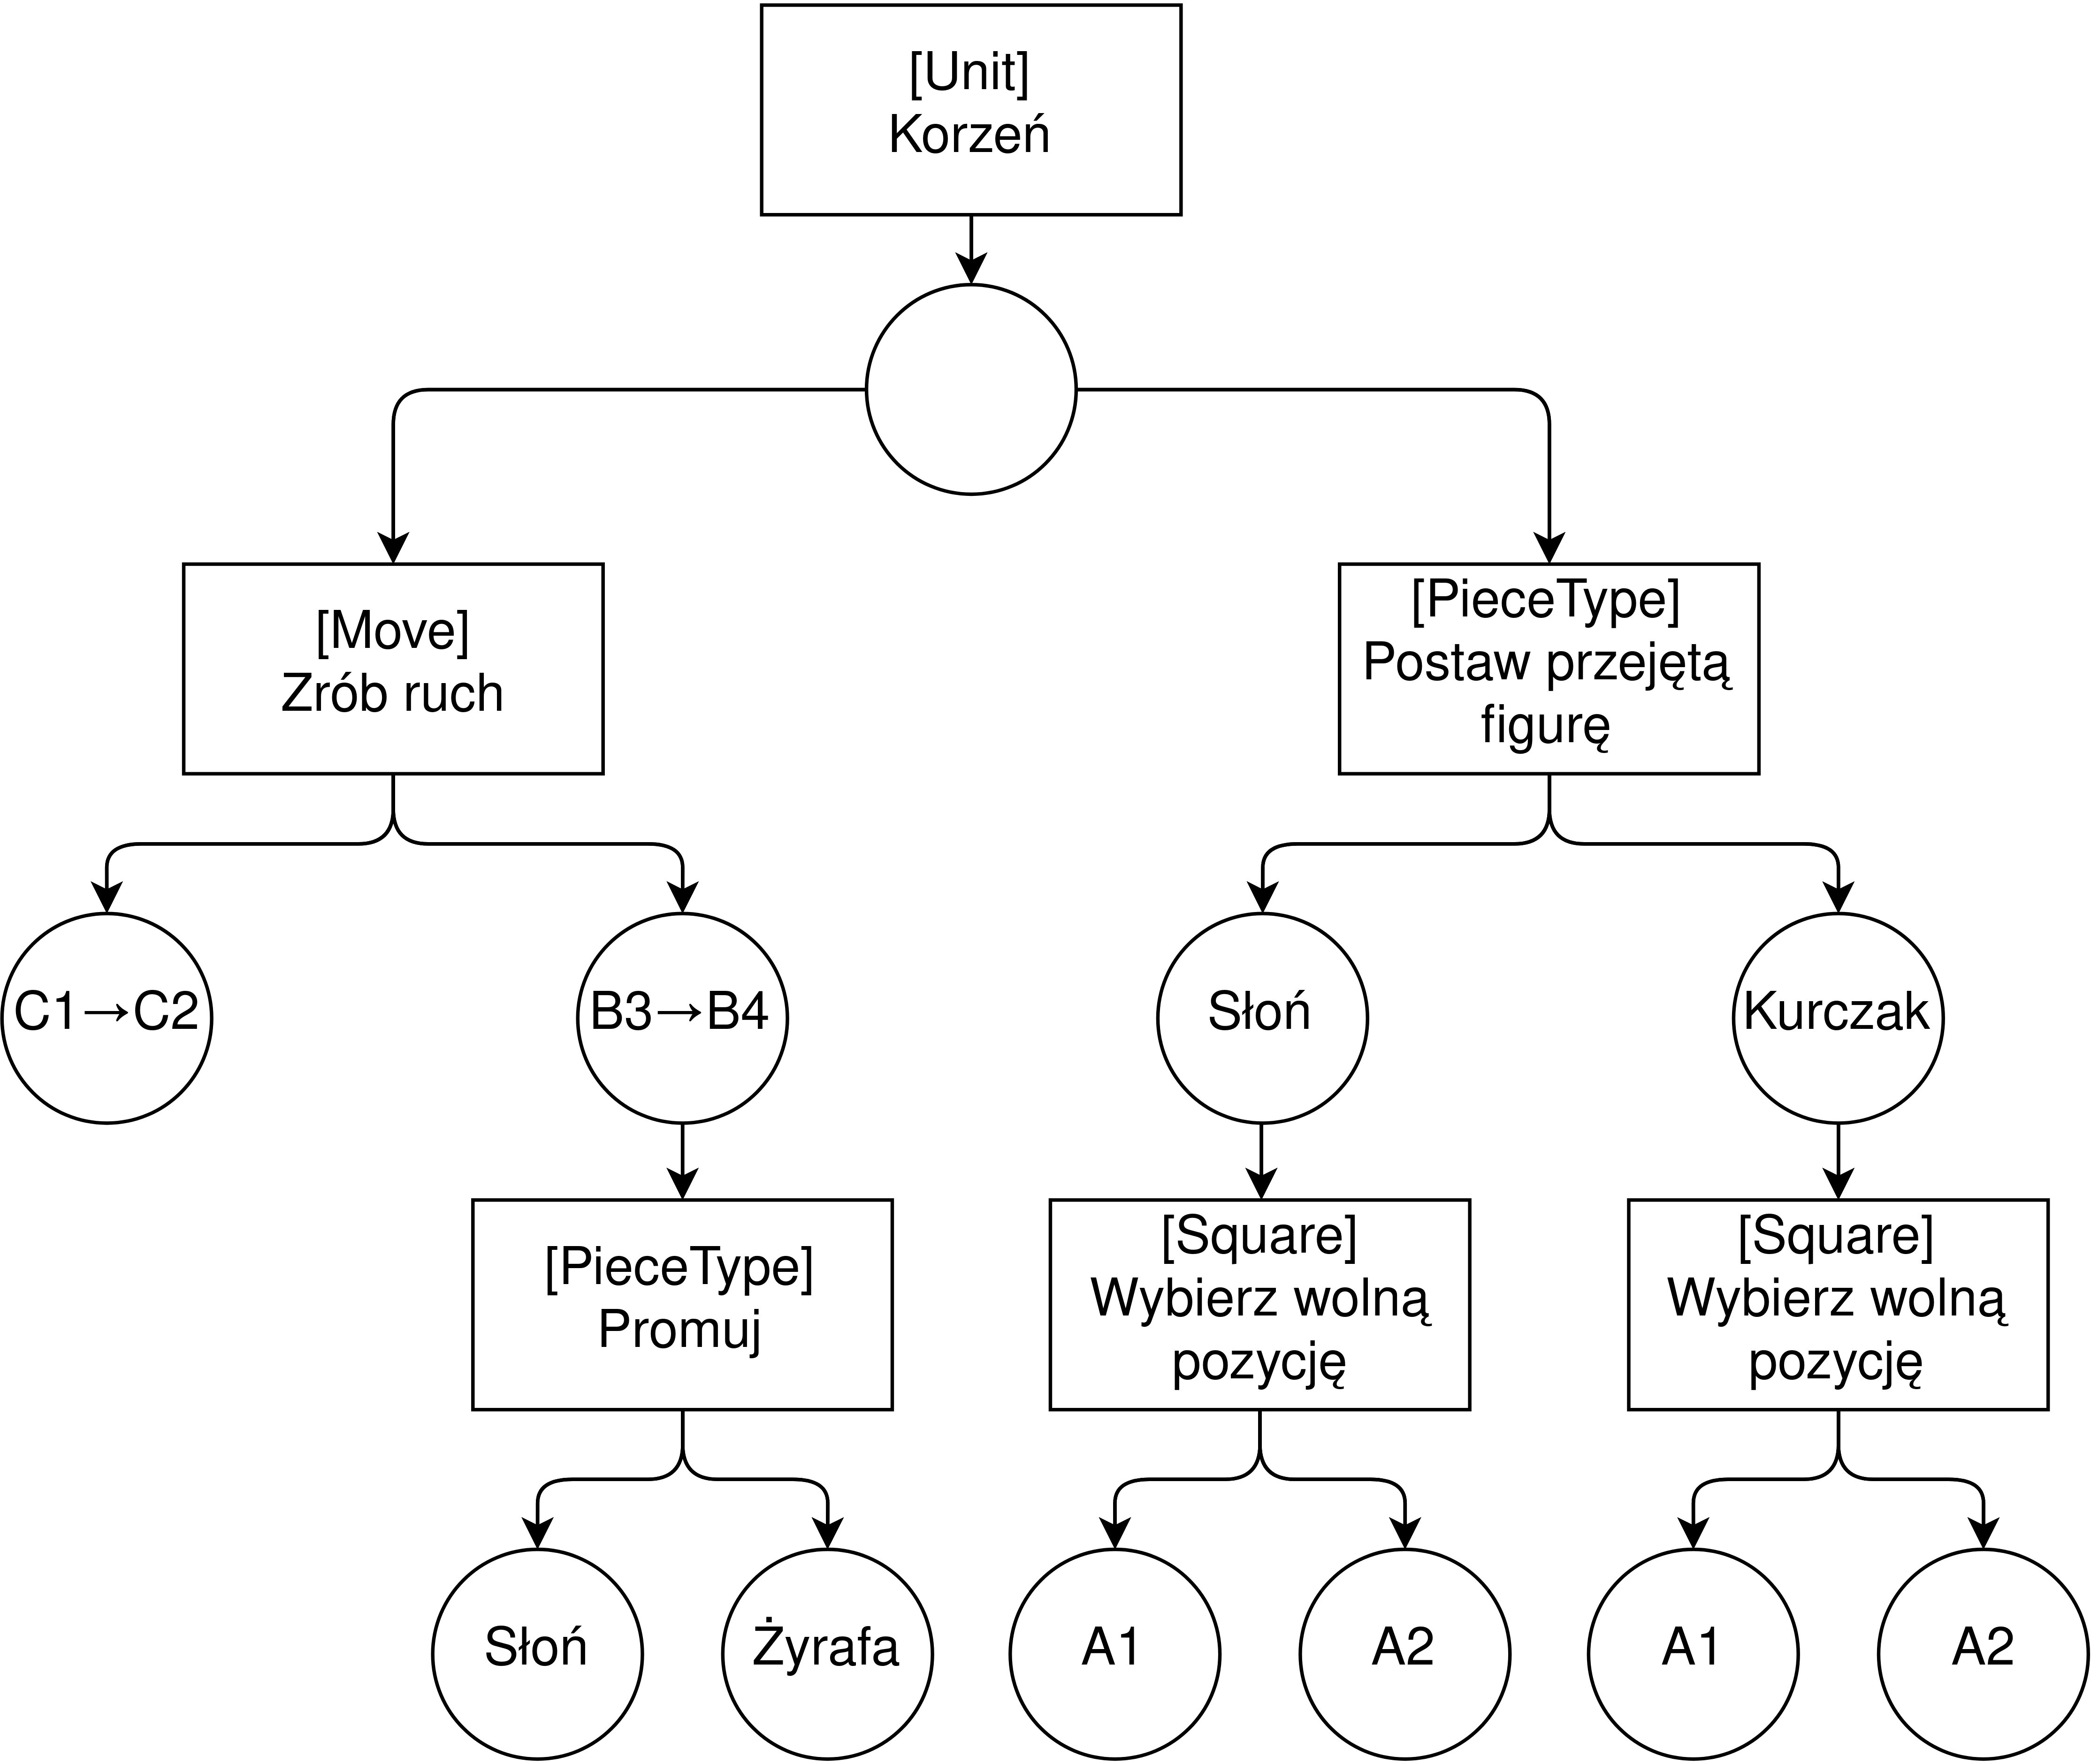
\includegraphics[height=7cm]{img/mess-option-diagram.jpg}
% 		\centering
% 	\end{figure}
% \end{frame}
%
% \begin{frame}[noframenumbering]
% 	\frametitle{Interakcja z użytkownikiem -- walidacja stanów}
% 	\begin{figure}
% 		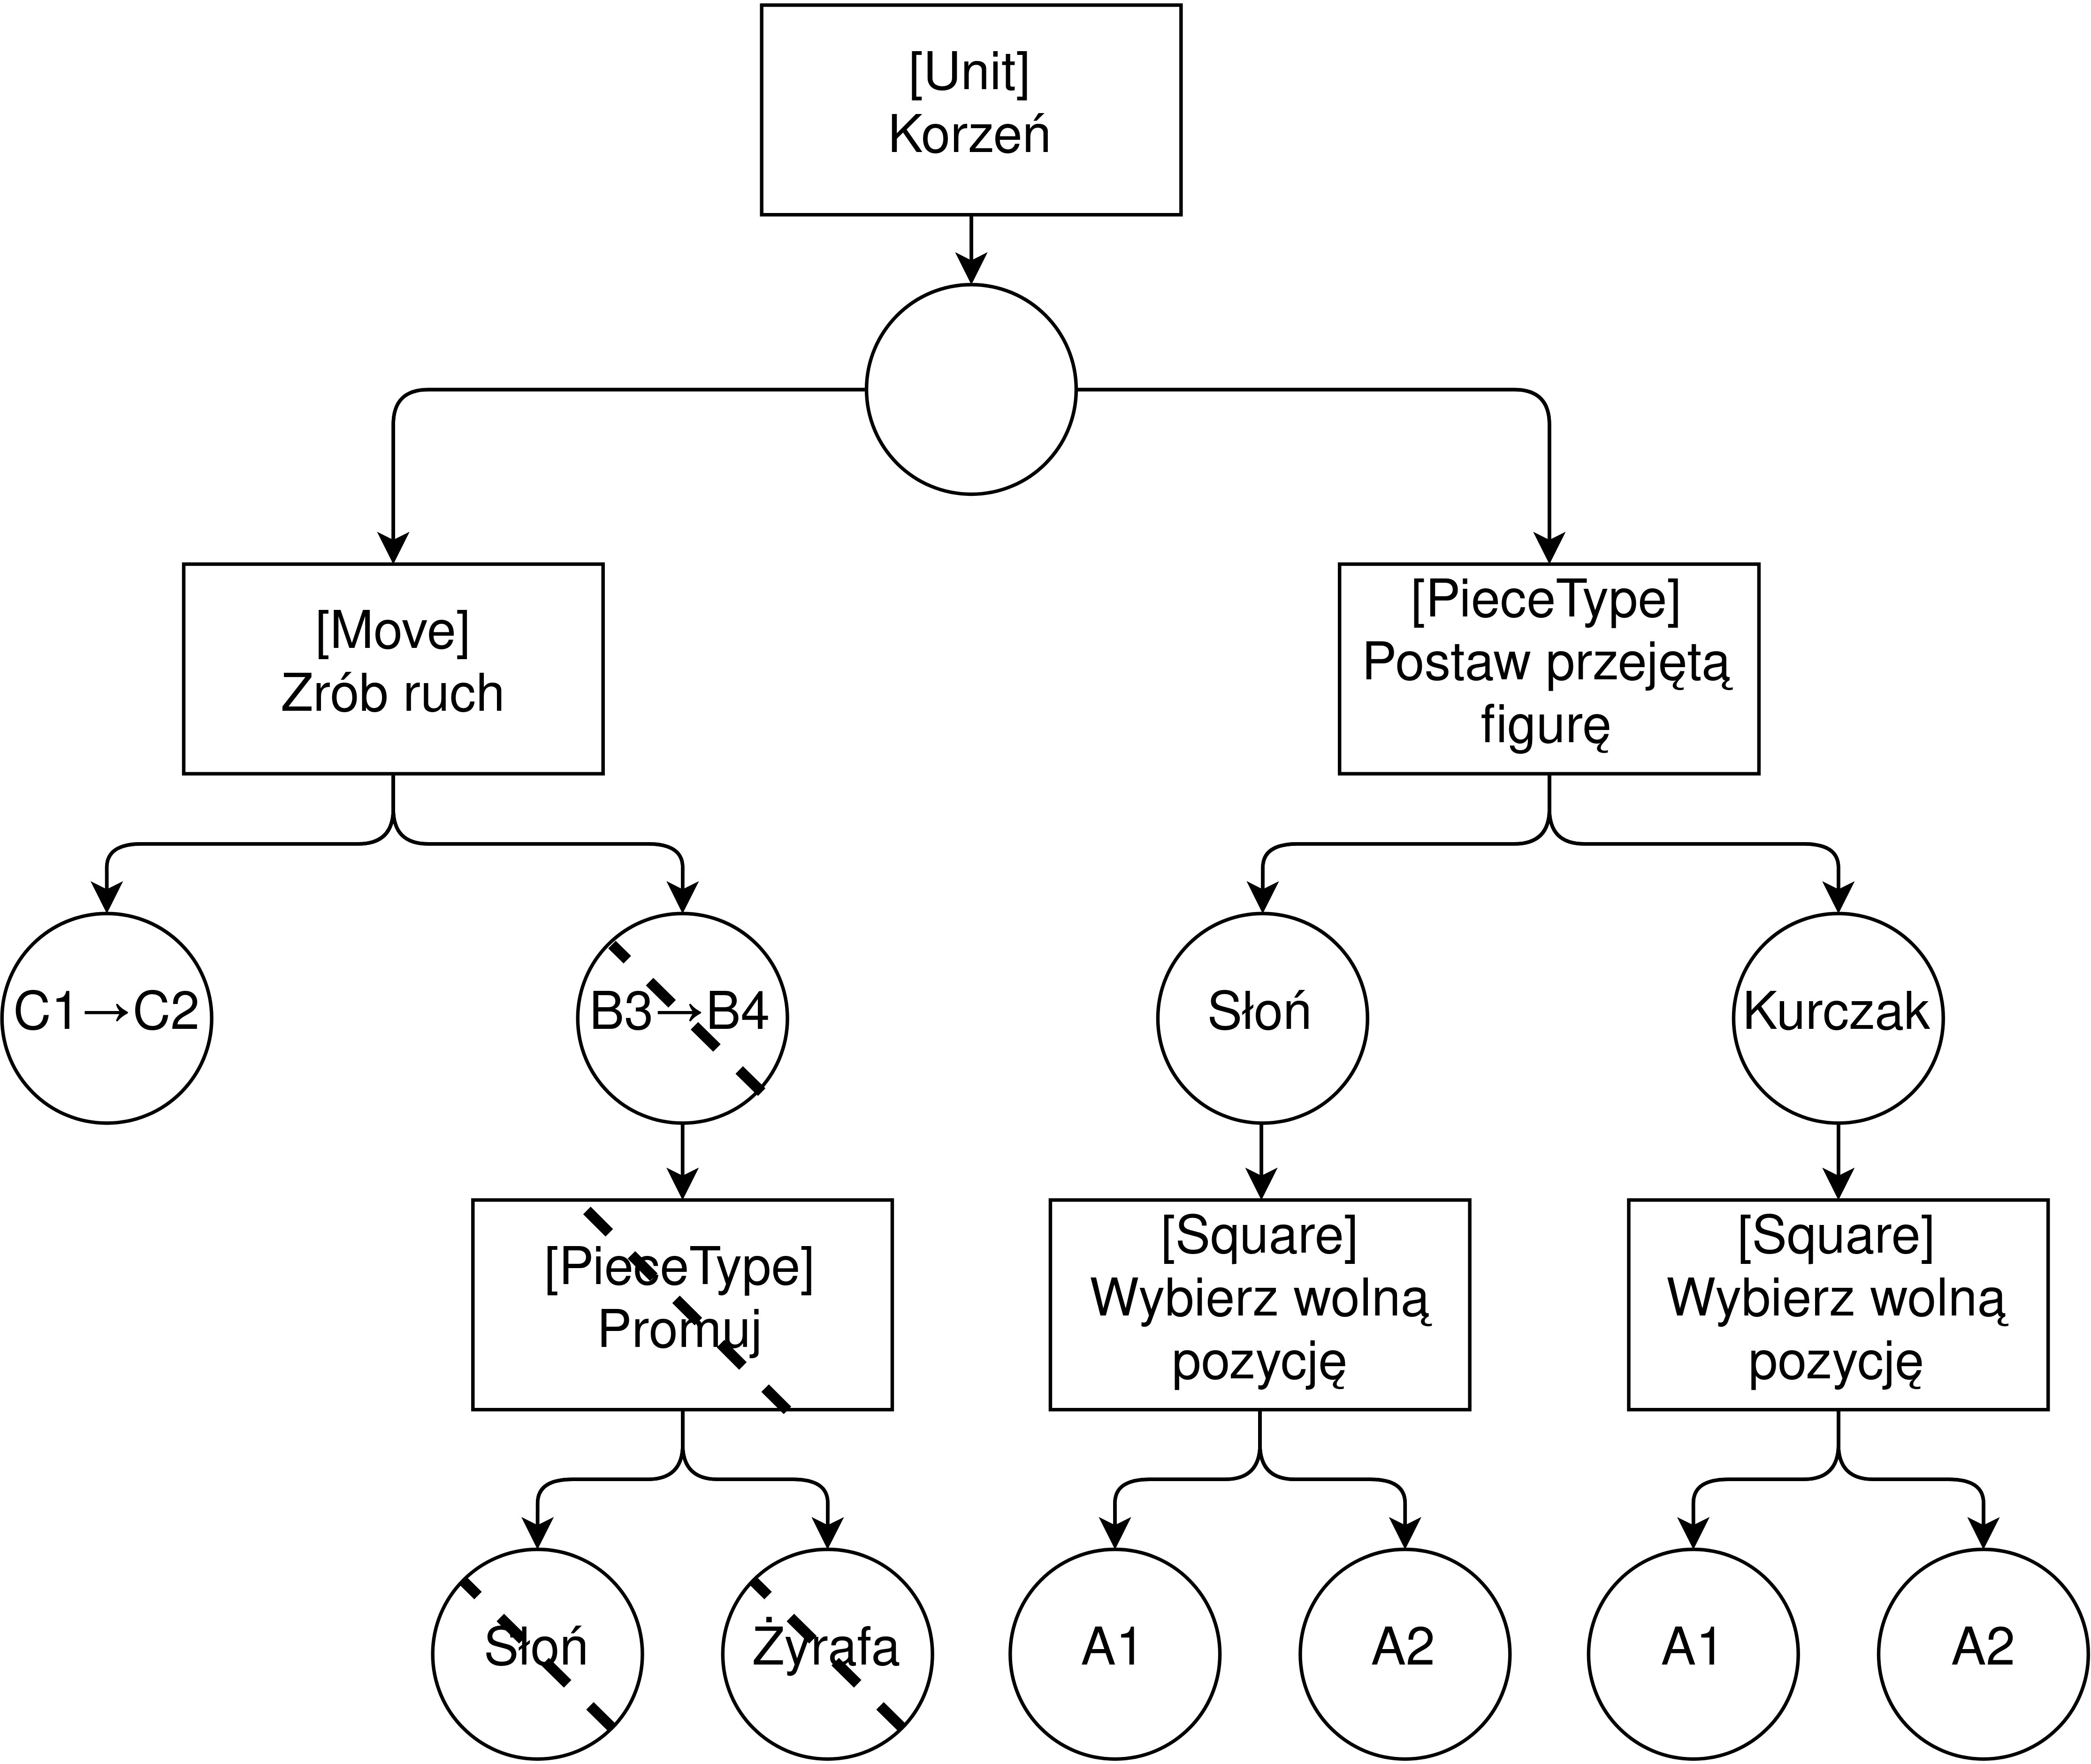
\includegraphics[height=7cm]{img/mess-validator-diagram.jpg}
% 		\centering
% 	\end{figure}
% \end{frame}

% \begin{frame}
% 	\frametitle{HCL bazą języka}
% 	Istniejący format HCL jako baza języka
% 	\begin{itemize}
% 		\item sprawdzony i znany format, używany m. in. w Terraformie\footnotemark
% 		\item zawiera elementy standardowych języków programowania:
% 		      \begin{itemize}
% 			      \item ewaluacja wyrażeń arytmetycznych i logicznych
% 			      \item wykonywanie funkcji wbudowanych
% 			      \item pętle w postaci ,,list/obiektów składanych'' (\emph{ang.} list/object comprehension)
% 		      \end{itemize}
% 		\item oficjalny dodatek {\tt userfunc} umożliwia definicję funkcji przez użytkownika
% 		\item zwięzły i czytelny kod
% 	\end{itemize}
% 	\footnotetext{Terraform -- narzędzie do zarządzania infrastrukturą komputerową w modelu infrastruktura jako kod (\emph{ang.} IaC -- Infrastructure as Code)}
% \end{frame}
%
% \begin{frame}[fragile]
% 	\frametitle{Język -- przykładowy kod (definicja typu figury)}
%
% 	\begin{lstlisting}
%   piece_type "pawn" {
%     motion {
%       generator = "motion_forward"
%       choice    = "promote_choose_piece_type"
%       action    = "promote"
%     }
%     motion {
%       generator = "motion_forward_double"
%     }
%     motion {
%       generator = "motion_forward_diagonal"
%       choice    = "promote_choose_piece_type"
%       action    = "promote"
%     }
%     motion {
%       generator = "motion_en_passant"
%       action    = "capture_en_passant"
%     } }
% 	\end{lstlisting}
% \end{frame}
%
% \begin{frame}[fragile]
% 	\frametitle{Język -- przykładowy kod (generator ruchu)}
%
% 	\begin{lstlisting}
% composite_function "motion_forward" {
%   params = [square, piece]
%   result = {
%     forward = owner_of(piece).forward_direction
%     dest = get_square_relative(square, forward)
%     return = dest == null ? [] : piece_at(dest) != null ? [] : [dest]
%   }
% }
%     \end{lstlisting}
% \end{frame}
%
% \begin{frame}[fragile]
% 	\frametitle{Język -- przykładowy kod (funkcja wyboru)}
% 	\begin{lstlisting}
% composite_function "promote_choose_piece_type" {
%   params = [piece, src, dst]
%   result = {
%     choice = {
%       message = "Promote"
%       type    = "piece_type"
%       options = [
%         for type in piece_types : type.name
%         if !contains(["king","pawn"], type.name)
%       ]
%     }
%     return = is_moving_to_last_rank(piece, dst) ? choice : null
%   }
% }
% 	\end{lstlisting}
% \end{frame}
%
% \begin{frame}[fragile]
% 	\frametitle{Język -- przykładowy kod (akcja)}
% 	\begin{lstlisting}
% composite_function "promote" {
%   params = [piece, src, dst, options]
%   result = {
%     owner = owner_of(piece)
%     piece_type = length(options) == 0 ? null : options[0].piece_type
%     _ = piece_type == null ? null : place_new_piece(piece_type.name, dst, owner.color)
%   }
% }
% 	\end{lstlisting}
% \end{frame}

% \begin{frame}%[allowframebreaks]
% 	\frametitle{Pozostałe ustalenia}
% 	\begin{itemize}
% 		% \item Język:
% 		%       \begin{itemize}
% 		% 	      \item opracowanie wstępnego pliku zasad przed pracami nad silnikiem i modyfikacja w miarę potrzeb
% 		% 	      \item moduł dekodujący, sprowadzający do obiektów domenowych używanych w silniku
% 		% 	      \item testy plików zasad w postaci testów integracyjnych
% 		%       \end{itemize}
% 		\item Silnik:
% 		      \begin{itemize}
% 			      \item język: Go (w nim jest napisany parser HCL)
% 			    %   \item testy jednostkowe silnika w odosobnieniu od modułu dekodującego zasady
% 			      \item komunikacja między obiektami za pomocą zdarzeń % (łatwa implementacja cofania ruchów)
% 		      \end{itemize}
% 		    %   \framebreak
% 		\item Interfejs użytkownika:
% 		      \begin{itemize}
% 			      \item początkowo tymczasowy interfejs terminalowy
% 			      \item docelowo interfejs w przeglądarce
% 			      \item TypeScript + React
% 			      \item komunikacja z silnikiem za pomocą protokołu HTTP oraz WebSocket
% 		      \end{itemize}
% 	\end{itemize}
% \end{frame}

% \section{Wyniki pracy}

% \begin{frame}
% 	\frametitle{Wyniki pracy}
% 	\begin{itemize}
% 		\item Stworzenie działającego systemu
% 		\item Konteneryzacja, wdrożenie na klaster Kubernetesa: \url{mess.westeurope.cloudapp.azure.com}
% 		\item Film demonstracyjny
% 		\item Możliwości rozwoju:
% 		      \begin{itemize}
% 			      \item poprawa wydajności obliczania dozwolonych przejść
% 			      \item dodanie kont użytkownika, repozytorium zasad
% 		      \end{itemize}
% 	\end{itemize}
% \end{frame}

% \begin{frame}
% 	\frametitle{Interfejs terminalowy -- szachy}
% 	\centering
% 	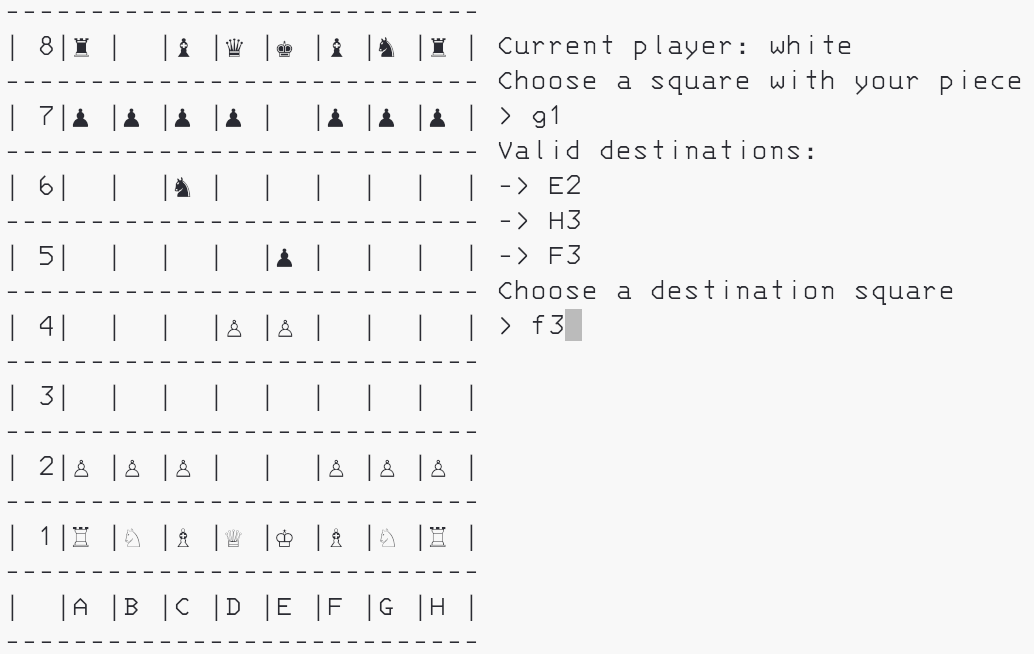
\includegraphics[width=0.95\textwidth]{img/chess-terminal.png}
% \end{frame}

% \begin{frame}
% 	\frametitle{Interfejs terminalowy -- Halma}
% 	\centering
% 	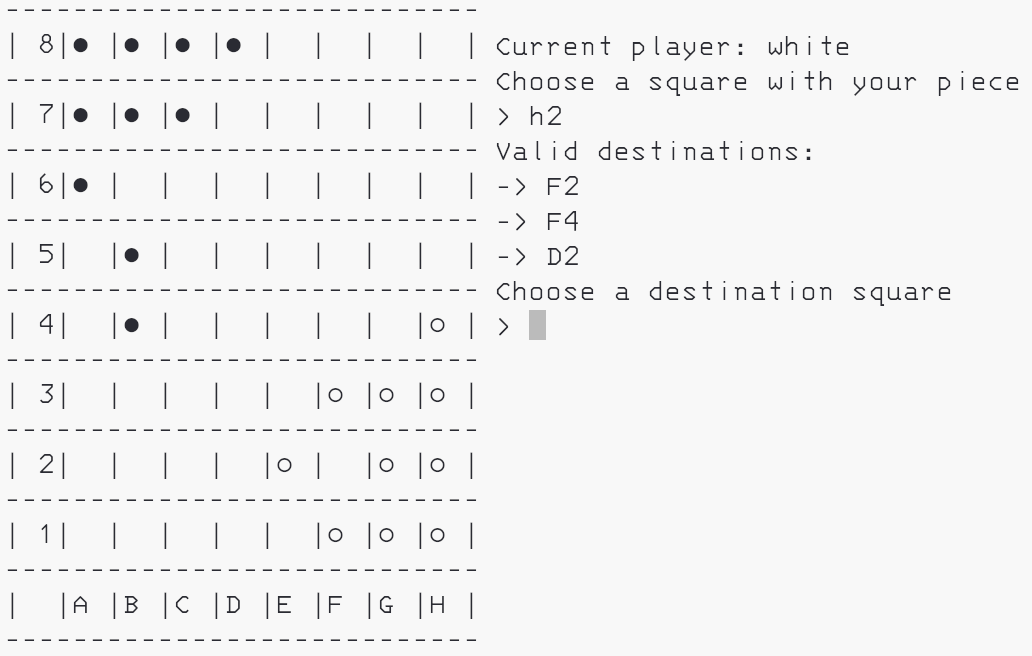
\includegraphics[width=0.95\textwidth]{img/halma-terminal.png}
% \end{frame}

% \begin{frame}
% 	\frametitle{Interfejs terminalowy -- Dōbutsu shōgi}
% 	\centering
% 	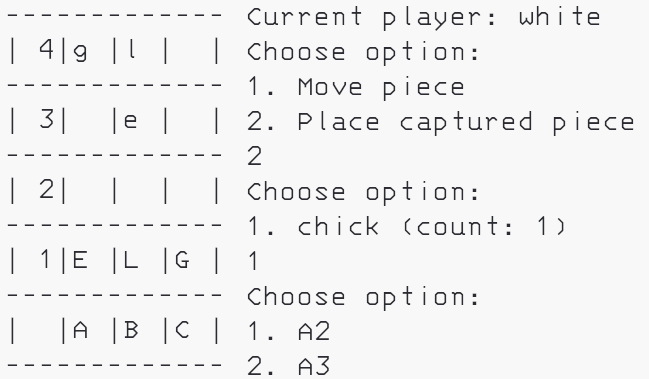
\includegraphics[width=0.95\textwidth]{img/dobutsu-shogi-terminal.png}
% \end{frame}

% \begin{frame}
% 	\frametitle{Interfejs w przeglądarce -- szachy}
% 	\centering
% 	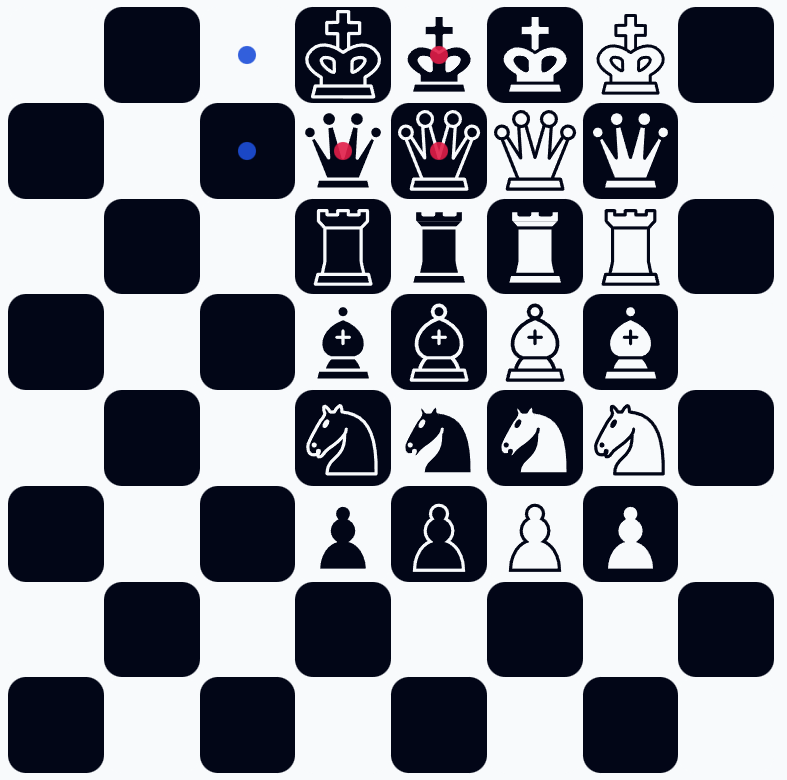
\includegraphics[height=0.85\textheight]{img/chess-browser.png}
% \end{frame}

% \section{Plan przyszłych prac}

% \begin{frame}
% 	\frametitle{Program minimum (gotowy)}
% 	\begin{itemize}
% 		\item Opracowanie języka dziedzinowego, bazującego na HCL, do opisywania zasad dwuosobowych gier planszowych opartych o szachownicę
% 		\item Język musi pozwalać na opisanie zasad:
% 		      \begin{itemize}
% 			      \item standardowych szachów
% 			      \item gry Dōbutsu Shōgi
% 			      \item gry Halma
% 		      \end{itemize}
% 		\item Projekt i implementacja silnika gry, będącego interpreterem ww. języka,
% 		\item Stworzenie interfejsu użytkownika, pozwalającego na prowadzenie rozgrywki dwóch osób
% 	\end{itemize}
% \end{frame}

% \begin{frame}
% 	\frametitle{Plan przyszłych prac}
% 	\begin{itemize}
% 		\item Październik:
% 		      \begin{itemize}
% 			      \item Stworzyć serwer HTTP/WS do interakcji z silnikiem
% 			      \item Połączyć interfejs w przeglądarce z ww. serwerem
% 		      \end{itemize}
% 		\item Listopad:
% 		      \begin{itemize}
% 			      \item Dodać możliwość gry na wielu urządzeniach
% 			      \item Rozszerzyć plik z zasadami o możliwość konfiguracji wyglądu figur
% 		      \end{itemize}
% 		\item Grudzień i styczeń
% 		      \begin{itemize}
% 			      \item Napisać pracę inżynierską
% 		      \end{itemize}
% 	\end{itemize}
% \end{frame}
%
% \begin{frame}
% 	\frametitle{Dodatkowe zagadnienia do rozwiązania}
% 	\begin{itemize}
% 		\item Zwiększyć poziom pokrycia kodu testami
% 		\item Zautomatyzować budowanie projektu (konteneryzacja)
% 		\item Wdrożyć projekt na wybraną usługę chmurową
% 		\item Dodać edytor tekstowy zasad do interfejsu w przeglądarce
% 		\item Dodać przyjazny edytor graficzny zasad do interfejsu w przeglądarce
% 	\end{itemize}
% \end{frame}

% \section{Wnioski}

% \begin{frame}
% 	\frametitle{Wnioski}
%
% 	\begin{itemize}
% 		\item Język dziedzinowy do generowania gier planszowych opartych o szachownicę
% 		\item Język bazuje na HCL, charakteryzuje się prostotą pisania i modyfikowania reguł oraz zwięzłością
% 		\item Opis zasad gry za pomocą funkcji ułatwia rozumienie kodu
% 	\end{itemize}
% \end{frame}
%
% \begin{frame}[allowframebreaks,noframenumbering]
% 	\frametitle{Bibliografia}
% 	\nocite{*} % Print all entries
% 	\printbibliography[heading=none]
% \end{frame}
%
%
% \begin{frame}[noframenumbering]
% 	\frametitle{Testy}
% 	\begin{itemize}
% 		\item Silnik testowany jednostkowo
% 		\item Moduł dekodujący i pliki zasad testowane integracyjnie, wraz z silnikiem
% 		\item Serwis API testowany integracyjnie wraz z pozostałymi komponentami
% 		\item Testy manualne
% 	\end{itemize}
% \end{frame}

% \begin{frame}[allowframebreaks,noframenumbering]
% 	\frametitle{Język -- podejścia}
% 	Możliwe podejścia:
% 	\begin{enumerate}
% 		\item stworzenie własnego języka dziedzinowego
% 		      \begin{itemize}
% 			      \pro całkowita możliwość dostosowania języka do potrzeb
% 			      \con tworzenie parsera bardzo pracochłonne
% 			      \con brak dodatkowych narzędzi (formatowanie, detekcja błędów składniowych, itp.)
% 			      \con brak znajomości języka u użytkowników
% 		      \end{itemize}
% 		\item stworzenie języka dziedzinowego zanurzonego w języku programowania (np. Kotlin, Haskell, Lua)
% 		      \begin{itemize}
% 			      \pro dostępne wszystkie możliwości języka nadrzędnego
% 			      \pro znajoma składnia dla użytkowników
% 			      \con trudny do ograniczenia (problem bezpieczeństwa)
% 		      \end{itemize}
% 		      \framebreak
% 		\item użycie istniejącego formatu (np. {\tt JSON}, {\tt YAML})
% 		      \begin{itemize}
% 			      \pro formaty popularne i znane przez użytkowników
% 			      \pro brak potrzeby tworzenia parsera
% 			      \con brak łatwego zapisu wyrażeń, funkcji, pętli, itp.
% 			      \con brak możliwości modyfikacji składni języka
% 		      \end{itemize}
% 	\end{enumerate}
% \end{frame}

% \begin{frame}[noframenumbering]
% 	\frametitle{HCL -- problemy}
% 	\begin{itemize}
% 		\item Dodatek {\tt userfunc} umożliwia tworzenie jedynie funkcji składających się z jednego wyrażenia
% 		      \begin{itemize}
% 			      \item rozwiązanie -- modyfikacja dodatku do potrzeb
% 		      \end{itemize}
% 		\item Ewaluacja operacji logicznych {\tt \&\&} i {\tt ||} nie jest ,,leniwa''
% 		      \begin{itemize}
% 			      \item niespodziewane błędy podczas interpretacji reguł
% 			      \item \lstinline|isValid = destination != null && piece_at(destination) == null|
% 		      \end{itemize}
% 	\end{itemize}
% \end{frame}


\end{document}
